
% Use the following line _only_ if you're still using LaTeX 2.09.
%\documentstyle[icml2014,epsf,natbib]{article}
% If you rely on Latex2e packages, like most moden people use this:
\documentclass{article}

% use Times
\usepackage{times}
% For figures
\usepackage{graphicx} % more modern
%\usepackage{epsfig} % less modern
\usepackage{subfigure}

% For citations
\usepackage{natbib}

% For algorithms
\usepackage{algorithm}
\usepackage{algorithmic}

% As of 2011, we use the hyperref package to produce hyperlinks in the
% resulting PDF.  If this breaks your system, please commend out the
% following usepackage line and replace \usepackage{icml2014} with
% \usepackage[nohyperref]{icml2014} above.
\usepackage{hyperref}

% Packages hyperref and algorithmic misbehave sometimes.  We can fix
% this with the following command.
\newcommand{\theHalgorithm}{\arabic{algorithm}}

% Employ the following version of the ``usepackage'' statement for
% submitting the draft version of the paper for review.  This will set
% the note in the first column to ``Under review.  Do not distribute.''
%\usepackage{icml2014}
% Employ this version of the ``usepackage'' statement after the paper has
% been accepted, when creating the final version.  This will set the
% note in the first column to ``Proceedings of the...''
\usepackage[accepted]{icml2014}

\usepackage{amsmath}
\usepackage{tikz}
\usetikzlibrary{arrows,positioning}

\newcommand{\D}{\mathcal{D}}
\newcommand{\ly}{\hat{y}(x;\D)}
\newcommand{\xt}{\tilde{x}}
\newcommand{\yt}{\tilde{y}}
\newcommand{\hht}{\tilde{h}}
\newcommand{\st}{\tilde{\sigma}}
\newcommand{\mut}{\tilde{\mu}}
\newcommand{\E}[1]{\left< #1 \right>}
\newcommand{\so}{\sigma_{\hat{y}}^2}
\newcommand{\sn}{\left< \tilde{\sigma}_{\hat{y}}^2 \right>}
\newcommand{\screenshot}[2]{\centerline{%
  \includegraphics[width=#1\textwidth,keepaspectratio]{../pics/#2}}}


% The \icmltitle you define below is probably too long as a header.
% Therefore, a short form for the running title is supplied here:
\icmltitlerunning{Summary Paper: Active Learning with Statistical Models}

\begin{document}

\twocolumn[
\icmltitle{Summary Paper: Active Learning with Statistical Models\\
by D. A. Cohn, Z. Ghahramani, M. I. Jordan}
% It is OKAY to include author information, even for blind
% submissions: the style file will automatically remove it for you
% unless you've provided the [accepted] option to the icml2014
% package.
\icmlauthor{Steffen Fuchs}{st.fuchs.tr@gmail.com}

% You may provide any keywords that you
% find helpful for describing your paper; these are used to populate
% the "keywords" metadata in the PDF but will not be shown in the document
\icmlkeywords{boring formatting information, machine learning, ICML}
\vskip 0.3in
]


\begin{abstract}
Active Learning has shown its great value in situations where data is expensive
or difficult to obtain. Cohn et al. \yrcite{Cohn96} describe how the prinicipal of
optimal data selection for neural networks can also be applied to two
alternative, statistically-based learning models, namely mixures of Gaussians
and locally weighted regression. This paper summarizes their proposal of a variance
reduction criteria for optimal data selection, reviews their experimental results
and discusses it within the contex of previous and subsequent work.
\end{abstract}

\section{Introduction}
In the research field of machine learning most often the algorithm is treated as a passive
recipient of the data it is supposed to learn from. However, in many situations
a learner also has the ability to act, to gather data and to influence
the world it is trying to understand. For example, in face recognition the
algorithm can query a human to tag or verify an unknown face. In robotics the
robot can move and use its sensors in order to learn the environment. Active
learning is the study of how to use this ability effectively and how to improve
performance with less training.

The biggest advantages are provided when using active learning on problems where
the acquistion of data is expensive or difficult. Hireing an expert of a
natural language for labeling words for speech recognition is time consuming
and expensive, therefore you might want to select these queries in an optimal way.

The authors differentiate between different goals for which active learning can be
used. One is optimization, where the algorithm performs experiments
in order to find the input values which give an optimal response. The authors
state that a common way to address this problem is a form of response surface
methodology\cite{box1987}, which performs experiments that guide hill-climbing
through the input space.

Another goal is to learn a control policy by taking certain actions which is
a common problem in the field of adaptive control or reinforcement learning.
An important requirement is to already perform well during learning. In
this case the learner has to decide on the trade-off between exploitation of
the current policy and exploration of new and hopefully better policies.

A third one is the problem of supervised learning which tries to accurately
predict a value $y$ for a given input $x$ based on a set of potenially noisy
samples. The work of the authors only addressed issues of the last kind.
The requirements are defined so that the learner itself is able to iteratvely select
a new input $\xt$ for which the resulting true output $\yt$ can be observed and
then used as a new sample for training. The task of active learning is to provide
a way of how to choose the next $\xt$.

\subsection{Related Work}
\label{sec:work}
By the time the article was published there existed several different heuristics
for choosing $\xt$. This includes choosing locations where no data exists
\cite{whitehead1991study}, locations with poor performance \cite{linden1993implementing},
locations with low confidence \cite{thrun1991active}, locations that are
expected to change the model \cite{cohn1994improving} and locations where data
was found previously and resulted in learning \cite{storck1995reinforcement}.
The heuristic chosen by the authors is to select $\xt$ in a statistically
``optimal'' manner which has been applied before in the context of neural
networks \cite{mackay1992information}.



\section{Review: Statistically Optimal Data Selection}
The following section provides a brief review on optimal data selection as
a statstical approach and then summarizes the propasal of the authors how
this principal is applied to mixture of Gaussians and locally weighted regression.

At first $P(x,y)$ is defined as the unknown joint distribution over input $x$
and output $y$, and $P(x)$ is the known marginal distribution also called
input distribution. The learner's output on input $x$ and a given training set $\D$
is denoted as $\hat{y}(x,\D)$ (For readability, the explicit dependence on $x$
and $\D$ is dropped for the remainder of this paper).
Based on the work of Geman et al. \yrcite{geman1992neural} the expected error of
a learner is assumed to consist of the noise of the distribution itself,
the bias of the learner and the variance of the learner.
The first part is independet of the learner
and the second one was neglected by the authors, leaving only the learner's
variance.
\begin{equation}
  \so = E \left[\left(\hat{y} - E \left[\hat{y}\right]\right)^2 \right]
\end{equation}
When a new input $\xt$ is selected and queried, and the resulting pair $(\xt,\yt)$
is added to the training set, $\so$ should change.
The learner's expected new variance is denoted $\sn$ where
$\left< \cdot \right>$ is the expectation given a fixed $x$-component of $\D$.

\begin{figure}\centering\small
  \begin{tikzpicture}[
    box/.style={rectangle,draw=black!80,thick,fill=blue!10,
      inner sep=5pt, minimum height=0.8cm, anchor=north},
    to/.style={->, >=stealth'},
    every node/.style={align=center}]

  \newcommand{\sep}{5pt}
  \node[box,fill=black!10] (init) {create initial sample};
  \node[box,below=\sep of init] (trai) {train new model from data $\D$};
  \node[box,below=\sep of trai] (refr) {from $P(x)$ draw $n$ reference points $x$};
  \node[box,below=\sep of refr] (cand) {generate a set of $m$ candidate points $\xt$ randomly \\
    (or select queries by hillclimbing on ${\partial\E{\st_{y|x}^2}}/{\partial\xt}$)};
  \node[box,below=\sep of cand] (avgv) {for each query point $\xt$ integrate
    $\E{\st_{\hat{y}}^2}$ \\ over all reference points (Monte Carlo integration)};
  \node[box,below=\sep of avgv] (minx) {query at $\xt$ with minimal average variance and\\
    add a new sample to training data $\D$};

  \path (init.south) edge[to] (trai.north);
  \path (trai.south) edge[to] (refr.north);
  \path (refr.south) edge[to] (cand.north);
  \path (cand.south) edge[to] (avgv.north);
  \path (avgv.south) edge[to] (minx.north);
  \draw[to] (minx.south) |- +(-4,-0.5) |-  (trai.west);

\end{tikzpicture}
\caption{Procedure proposed by the authors for optimal data selection}
\label{fig:proc}
\end{figure}


The goal is now to find an $\xt$ that minimizes $\sn$ when integraded over $X$.
To achive this, it is first assumed that the variance $\so$ of
the learner at $x$ is known. If, for some new input $\xt$ the conditional
distribution $P(\yt|\xt)$ is known, it would be possible to compute an
estimate of the learner's new variance at $x$. Although the true distribution
$P(\yt|\xt)$ is unknown, many learning models allow to approximate the output
distribution of $\yt$ in terms of mean and variance.

The average expected variance is then computed using Monte Carlo approximation,
evaluating $\sn$ at a number $n$ of reference points drawn according to $P(x)$.
To find the $\xt$ with minimal average expected variance for lower dimensional problems,
the authors suggested to simply evaluate it on a random set of candidate points.
Alternativly hillclimping on ${\partial\E{\st_{y|x}^2}}/{\partial\xt}$
can be used for higher dimensional problems. See Figure~\ref{fig:proc} for an
overview of the selection procedure.

The following parts show two examples proposed by the authors to first
approximate the output distribution $\yt$ at a new query $\xt$ and
from this to estimate the learner's new variance $\sn$ at $x$.

\subsection{Active Learning with a Mixture of Gaussians}
\begin{figure}\centering
  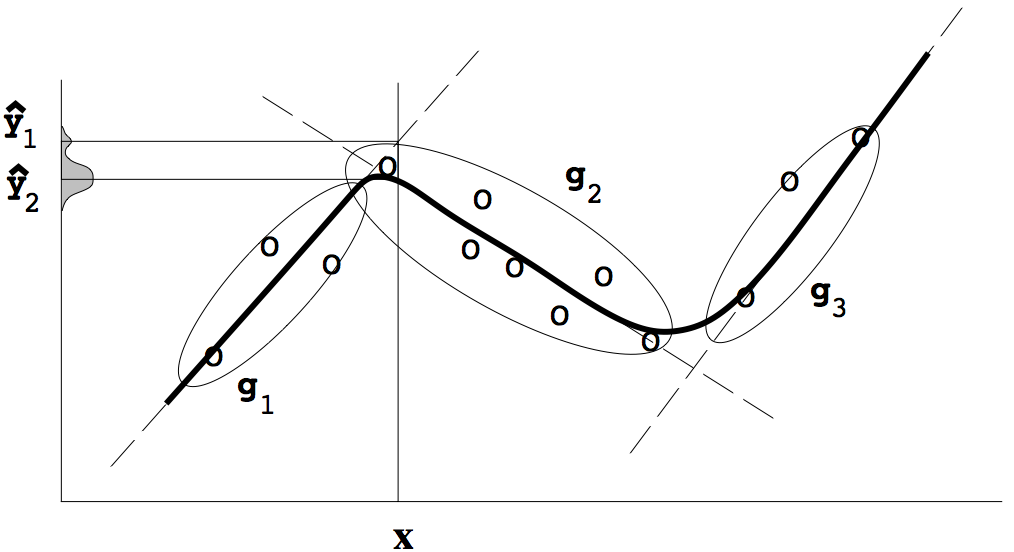
\includegraphics[width=1.0\columnwidth,keepaspectratio]{../pics/GMM.png}
  \caption{Using mixture of Gaussians to compute $\hat{y}$}
  \label{fig:gmm}
\end{figure}

In the context of learning, the mixture of Gaussians model assembles a joint
density estimation over the input/output space $X \times Y$ given the training
set $\D$ by fitting a defined number $N$ of mulitvariate Gaussians $g_i$ to it
(see Figure~\ref{fig:gmm}). The propability of a point $(x,y)$, given $g_i$ can
then be expressed as
\begin{equation}\small
P(x,y|i) = \frac{1}{2\pi\sqrt{|\Sigma_i|}} \exp
\left[ -\frac{1}{2}(\mathbf{x}-\mu_i)^T\Sigma_i^{-1}(\mathbf{x}-\mu_i) \right]
\end{equation}
with means and covariances as
\[
\mathbf{x} = \left[ \begin{array}{c} x \\ y \end{array} \right] \quad
\mu_i = \left[ \begin{array}{c} \mu_{x,i} \\ \mu_{x,i} \end{array} \right] \quad
\Sigma_i = \left[ \begin{array}{cc} \sigma^2_{x,i} & \sigma_{xy,i} \\
    \sigma_{xy,i} & \sigma^2_{y,i} \end{array} \right]
\]
which are usally estimated using the EM algorithm \cite{dempster1977maximum}.
These can then be used to compute the conditional expectation output $\hat{y}$
and its variance $\so$ for a certain $x$ and eventually lead to the new variance
$\sn$ at $x$ for a given query $\xt$. This can all be computed in closed form
using the following equations provide by the authors step by step:

\[\begin{split}
 \hat{y}_i &= \mu_{y,i} + \frac{\sigma_{xy,i}}{\sigma_{x,i}^2}(x-\mu_{x,i}),\\
 \sigma_{y|x,i}^2 &= \sigma_{y,i}^2 - \frac{\sigma_{xy,i}^2}{\sigma_{x,i}^2},\\
 h_i &\equiv h_i(x) = \frac{P(x|i)}{\sum_{j=1}^N P(x|j)},\\
 \hht_i &\equiv h_i(\xt),\\
 n_i &= \sum_{j=1}^m \frac{P(x_j,y_j|i)}{\sum_{k=1}^N P(x_j,y_j|k)},
\end{split}\]
\[\begin{split}
 \E{\st_{xy,i}} &= \frac{n_i\sigma_{xy,i}}{n_i+\hht_i} + \frac{n_i\hht_i
    (\xt-\mu_{x,i})(\hat{y}_i(\xt)-\mu_{y,i})} {(n_i+\hht_i)^2},\\
 \E{\st_{xy,i}^2} &= \E{\st_{xy,i}}^2 +
   \frac{n_i^2\hht_i^2\sigma_{y|\xt,i}^2(\xt-\mu_{x,i})^2}{(n_i+\hht_i)^4},\\
 \E{\st_{y,i}^2} &= \frac{n_i\sigma_{y,i}^2}{n_i+\hht_i} +
   \frac{n_i\hht_i\left(\sigma_{y|\xt,i}^2 + (\hat{y}_i(\xt)-\mu_{y,i})^2 \right)}
   {(n_i+\hht_i)^2},\\
 \E{\st_{y|x,i}^2} &= \E{\st_{y,i}^2} - \frac{\E{\st_{xy,i}^2}}{\sigma_{x,i}^2}
\end{split}\]
which can finally be used in
\begin{equation}
   \E{\st_{\hat{y}}^2} = \sum_{i=1}^N
   \frac{h_i^2 \E{\st_{y|x,i}^2}}{ (n_i+\hht_i)^2}
   \left( 1+\frac{(x-\mu_{x,i})^2}{\sigma_{x,i}^2} \right).
\end{equation}

\subsection{Active Learning with Locally Weighted Regression}
\begin{figure}\centering
  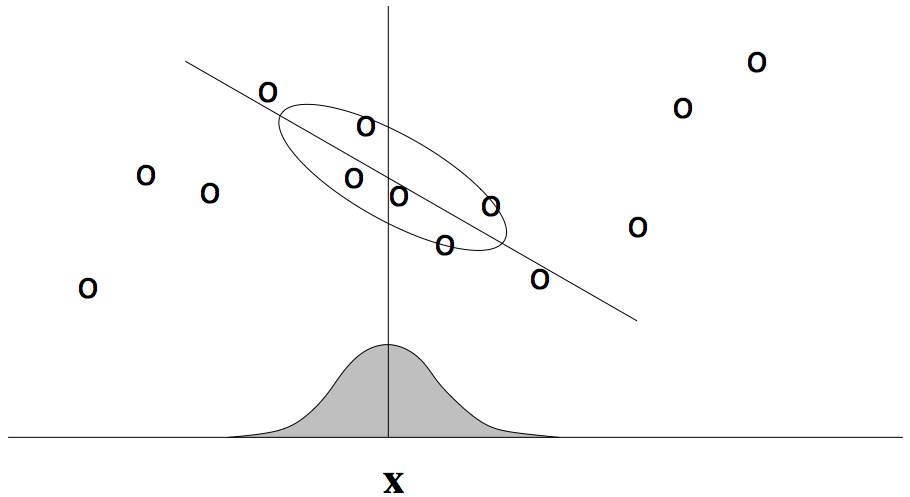
\includegraphics[width=1.0\columnwidth,keepaspectratio]{../pics/LWR.png}
  \caption{In locally weighted regression, the local neighborhood around $x$ is
  weighted by the kernel function (here Gaussian).
  Then linear regression is perfromed.}
  \label{fig:lwr}
\end{figure}
Locally weighted regression belongs to the family of lazy learners and
performs a regresssion using only training data in the local neighborhood
of the point of interest. The authors used a variant of the LOESS model
\cite{cleveland1988locally} which performs a linear regression on the
data set points weighted by a kernel centered at the query $x$
(see Figure~\ref{fig:lwr}). The kernel function is defined as
\begin{equation}
h_i(x) \equiv h(x-x_i) = \exp(-k(x-x_i)^2)
\end{equation}
with smoothing parameter $k$. The means and covariances at a desired $x$ can
then be estimated as
\begin{equation}\begin{split}
  \mu_x &= \frac{\sum_i h_ix_i}{n}, \quad
  \sigma_x^2 = \frac{\sum_i h_i(x_i-\mu_x)^2}{n}, \\
  \mu_y &= \frac{\sum_i h_iy_i}{n}, \quad
  \sigma_y^2 = \frac{\sum_i h_i(x_i-\mu_x)^2}{n}, \\
  \sigma_{xy} &= \frac{\sum_i h_i(x_i-\mu_x)(y_i-\mu_y)}{n}
\end{split}\end{equation}
with $n = \sum_i h_i$.

Similar to the case with mixture of Gaussian, one need compute $\sn$ in order
select the best $\xt$. Again the authors provide all necessary equations
required for a step by step computation:
\[\begin{split}
\mut_x &= \frac{n\mu_x+\hht\xt}{n+\hht},\\
\st_{x}^2 &= \frac{n\sigma_{x}^2}{n+\hht} + \frac{n \hht (\xt-\mu_{x})^2}{(n+\hht)^2},\\
\hat{y}(x) &= \mu_{y} + \frac{\sigma_{xy}}{\sigma_{x}^2}(x-\mu_{x}),\\
\sigma_{y|x}^2 &= \sigma_{y}^2 - \frac{\sigma_{xy}^2}{\sigma_{x}^2},
\end{split}\]
\[\begin{split}
\E{\st_{xy}} &= \frac{n\sigma_{xy}}{n+\hht} +
  \frac{n \hht (\xt-\mu_{x})(\hat{y}(\xt)-\mu_{y})}{(n+\hht)^2},\\
\E{\st_{xy}^2} &= \E{\st_{xy}}^2 +
  \frac{n^2\hht^2\sigma_{y|\xt}^2(\xt-\mu_{x})^2}{(n+\hht)^4},\\
\E{\st_{y}^2} &= \frac{n\sigma_{y}^2}{n+\hht} +
  \frac{n\hht \left( \sigma_{y|\xt}^2 + (\hat{y}(\xt)-\mu_{y})^2 \right)}
  {(n+\hht)^2}, \\
\E{\st_{y|x}^2} &= \E{\st_{y}^2} - \frac{\E{\st_{xy}^2}}{\sigma_{x}^2},
\end{split}\]
and eventually
\begin{small}
\begin{equation}\begin{split}
\E{\st_{\hat{y}}^2} =& \frac{\E{\st_{y|x}^2}}{(n+\hht)^2} \bigg[ \sum_i h_i^2 + \hht^2 \\
  +& \frac{(x-\mut_x)^2}{\st_x^2} \left( \sum_i h_i^2 \frac{(x_i - \mut_x)^2}{\st_x^2} +
    \hht^2 \frac{(\xt-\mut)^2}{\st_x^2} \right) \bigg].
\end{split}\end{equation}
\end{small}
\subsection{Experimental Results}
The authors evaluated their work on a 2-degree-of-freedom robot arm. The task
was to learn the kinematics, that means finding a mapping for input joint angles
to output Cartesian coordiantes of the tip. They compared the performance of
their proposed variance minimization criteria with a random selection of new
query points $\xt$ for both statistical models.

As expected, with increasing number of training samples, both models
showed significantly faster variance reduction of the
learner compared to a learner trained with the same number of samples but
selected randomly.
The same is true for the mean squared error which is also greatly smaller
than with random selection.

While the training time of Gaussian mixture model increases linearly with
the training set size, the time to select the next best $\xt$ is always constant.
Given the results of the authors for this experiment, it is interesting to see that with a set size of
around 30, the training time becomes the dominant factor and therefore makes
it infeasible for realtime application.
On the other hand locally weighted regression has no training time but for prediction
and selecting optimal data it increases linearly with training set size.
This also means choosing the training data wisely is double important.

\section{Discussion}
The authors have presented ways to perform active learning with two commonly used
and elegant learning algorithms. Their proposed criteria of variance minimization
for data selection can be computed efficently.
They also state that applying their approach to problems of classification
domain can be achived easily.

Although they mention several other criteria (see Section~\ref{sec:work}), they
miss out on the opportunity to actually compare them in theory as well as
within their experiments. A statement of how their method stands out against
others would have made a nice addition to their work.

Related to this work, Cohn et al.~\yrcite{cohn2003semi} developed a
semi-supervised clustering algorithm that uses feedback in order to learn
the clustering metric.
Tuia et al.\yrcite{tuia2009active} describe how to use active learning methods
for image classification on remote sensing devices (such as satellites).
Although their work features similarities to the variance reduction approach,
they apply active learning on support vector machines.
In fact in most cases when active learning is used for an actual application,
it is rather an classification problem than a function approximation and
the learning models considered here were not applied.


% In the unusual situation where you want a paper to appear in the
% references without citing it in the main text, use \nocite
%\nocite{langley00}

\bibliography{literature}
\bibliographystyle{icml2014}

\end{document}


